\documentclass{beamer}

\mode<presentation>
 {\usetheme{CambridgeUS}
  \usecolortheme{beaver}
  \setbeamercovered{transparent}
  % appearance of bullets
  \useinnertheme{rectangles}
  \definecolor{mybullets}{rgb}{0.6,0.0,0.0}
  \setbeamercolor{structure}{fg=mybullets}

  \definecolor{mycolor}{rgb}{0.2,0.2,0.2}
  % bars
  %\setbeamercolor{section in toc}{fg=black,bg=white}
  %\setbeamercolor{alerted text}{fg=mycolor!80!gray}
  %\setbeamercolor*{palette primary}{fg=mycolor!60!black,bg=gray!30!white}
  %\setbeamercolor*{palette secondary}{fg=mycolor!70!black,bg=gray!15!white}
  %\setbeamercolor*{palette tertiary}{bg=mycolor!80!black,fg=gray!10!white}
  %\setbeamercolor*{palette quaternary}{fg=mycolor,bg=gray!5!white}
  %\setbeamercolor*{sidebar}{fg=mycolor,bg=gray!15!white}

  \setbeamercolor*{palette sidebar primary}{fg=mycolor!10!black}
  \setbeamercolor*{palette sidebar secondary}{fg=white}
  \setbeamercolor*{palette sidebar tertiary}{fg=mycolor!50!black}
  \setbeamercolor*{palette sidebar quaternary}{fg=gray!10!white}

  \setbeamercolor{titlelike}{parent=palette primary,fg=mycolor}
  \setbeamercolor{frametitle}{bg=gray!10!white}
  \setbeamercolor{frametitle right}{bg=gray!60!white}

  \setbeamercolor*{separation line}{}
  \setbeamercolor*{fine separation line}{}
}

 \def\Tiny{\fontsize{5pt}{5pt}\selectfont}
 \renewcommand{\arraystretch}{1.2}

% just show sections and subsections in table of contents
\setcounter{tocdepth}{2}

\usepackage[english]{babel}
\usepackage[latin1]{inputenc}

\usepackage{times}
\usepackage[T1]{fontenc}

\usepackage{hyperref}

\newcommand{\foo}{\hspace{-2.3pt}$\bullet$ \hspace{5pt}}

\title[Profibus]{\textbf{Pro}cess \textbf{Fi}eld \textbf{Bus}}

\author[Koslowski]{Konstantin Koslowski (316955)}

\institute[]
{TU Berlin \\
 Department of Telecommunication Systems \\
 Telecommunication Networks Group \\
}

\date{June 19th, 2015}

\pgfdeclareimage[height=0.5cm]{university-logo}{tu-tkn-logo.jpg}
\logo{\pgfuseimage{university-logo}}

\begin{document}

\begin{frame}
  \titlepage
\end{frame}

\begin{frame}
\frametitle{Table of Contents}
\setcounter{tocdepth}{1}
\tableofcontents
\end{frame}

\section{Introduction}


\subsection{Development of Profibus}
\begin{frame}
\frametitle{Timeline}
\begin{itemize}
  \item Master development plan ``fieldbus'' created 1986 in Germany
  \item 21 companies, including Siemens, involved
  \item First promoted in 1989 by BMBF \textit{(Bundesministerium f\"ur Bildung und Forschung)}
  \item Goal: implement a bit-serial field bus for factory and process automation
    \begin{itemize}
      \item send one data bit at a time
      \item single wire
      \item opposed to bit-parallel word architectures
    \end{itemize}
  \item Published openly as part of IEC 61158 \textit{Digital data communication for measurement and
      control - Fieldbus for use in industrial control systems}
\end{itemize}
\end{frame}

\subsection{System Structure}
\begin{frame}
  \frametitle{System Structure - Introduction}
  \begin{itemize}
    \item Profibus is a multi-master system
    \item Operation of multiple systems over a single bus
    \item Three protocols available
      \begin{itemize}
        \item FMS \textit{(field-bus message specification)}
        \item DP \textit{(decentralized peripheral)}
        \item PA \textit{(process automation)}
      \end{itemize}
    \item Devices are categorized in different types
      \begin{itemize}
        \item Masters
        \item Slaves
      \end{itemize}
  \end{itemize}
\end{frame}

\begin{frame}
  \frametitle{System Structure - Layer}
  \begin{tabular}[h]{c|c|c}
    \textbf{Layer}  & \textbf{Name}     & \textbf{Content} \\
    \hline
    Layer 8         & User Layer        & Profiles \\
    Layer 7         & Application Layer & DP / FMS protocol \\
    Layer 2         & Data Link Layer   & FDL protocol \\
    Layer 1         & Physical Layer    & Transmission Technology
  \end{tabular} \\
  \hfill \\
  Profibus following the OSI reference model\cite{profibusmanual}
\end{frame}

\begin{frame}
  \frametitle{Protocol: FMS}
  \begin{itemize}
    \item FMS
  \end{itemize}<++>
\end{frame}

\begin{frame}
  \frametitle{Protocol: DP}
  \begin{itemize}
    \item DP
  \end{itemize}<++>
\end{frame}

\begin{frame}
  \frametitle{Protocol: PA}
  \begin{itemize}
    \item PA
  \end{itemize}<++>
\end{frame}

\begin{frame}
  \frametitle{Device Type: Master}
  \textbf{Masters}
  \begin{itemize}
    \item described as \textit{active stations}
    \item control the data traffic on the bus
    \item when having the \textit{bus access token}:\\
      send messages without external requests
  \end{itemize}
\end{frame}

\begin{frame}
  \frametitle{Device Type: Master}
  \textbf{Masters}
  \begin{itemize}
    \item described as \textit{active stations}
    \item control the data traffic on the bus
    \item when having the \textit{bus access token}:\\
      send messages without external requests
  \end{itemize}
\end{frame}

\begin{frame}
  \frametitle{Device Type: Slave}
  \begin{itemize}
    \item foo
  \end{itemize}<++>
\end{frame}

\begin{frame}
  \frametitle{Bus Access}
  \begin{itemize}
    \item via bus access token
  \end{itemize}<++>
\end{frame}


%
% \subsection{Network Topology}
% \begin{frame}
%   \frametitle{Network Topology}
%   \begin{itemize}
%     \item CAN networks use shared bus topology
%     \item Buses have to be terminated
%     \item Topology should be as linear as possible
%     \item Maximum bitrate and length directly dependent
%     \item No effective way to share line for power and signalling
%   \end{itemize}
% \end{frame}
%
% \begin{frame}
%   \frametitle{Transmission Medium}
%   Several kinds of transmission media can be used:
%   \begin{itemize}
%     \item \textbf{Two-wire bus}: Enables differential signal transmission, ensures reliable communication. Requirement for high-speed CAN.
%     \item \textbf{Single-wire bus}: Simpler/cheaper alternative, fall back in case of fault.
%     \item \textbf{Optical transmission medium}: Ensures immunity to electromagnetic noise, used to interconnect different subnets.
%   \end{itemize}
% \end{frame}
%
% \begin{frame}
%   \frametitle{ISO 11898-2: High-speed CAN}
%   \begin{itemize}
%     \item Maximum bit rate 1 Mbps
%     \item Linear bus end-terminated with $120 \Omega$
%     \item Stubs must be shorter than 30 cm
%   \end{itemize}
%   \begin{figure}
% 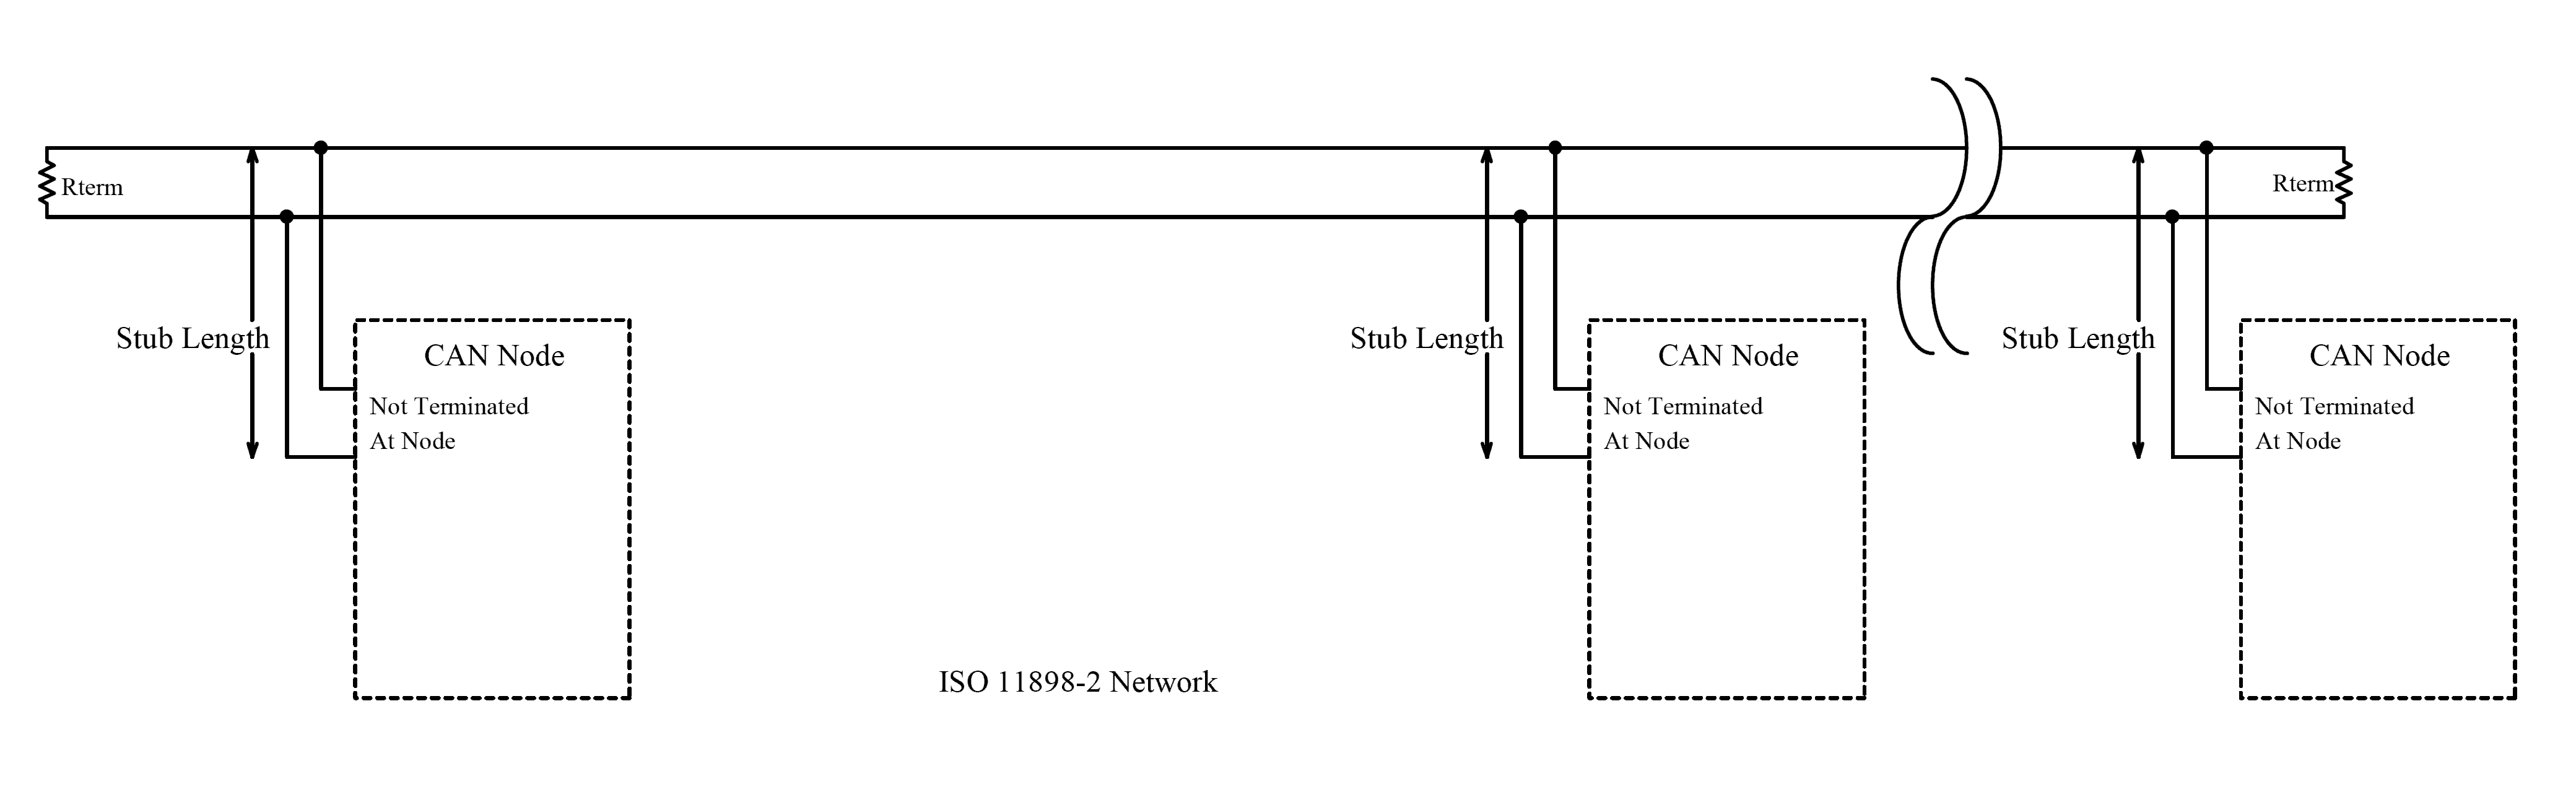
\includegraphics[width=.75\textwidth]{highspeed.png}
% \caption{High Speed CAN Network \cite{iso118982}}
% \end{figure}
% \end{frame}
%
% \begin{frame}
%   \frametitle{ISO 11898-3: Low-speed fault-tolerant CAN}
%   \begin{itemize}
%     \item Maximum bit rate 125 kbps
%     \item Linear or star bus terminated at node with about $100 \Omega$
%     \item Features energy-saving sleep mode
%   \end{itemize}
%   \begin{figure}
% 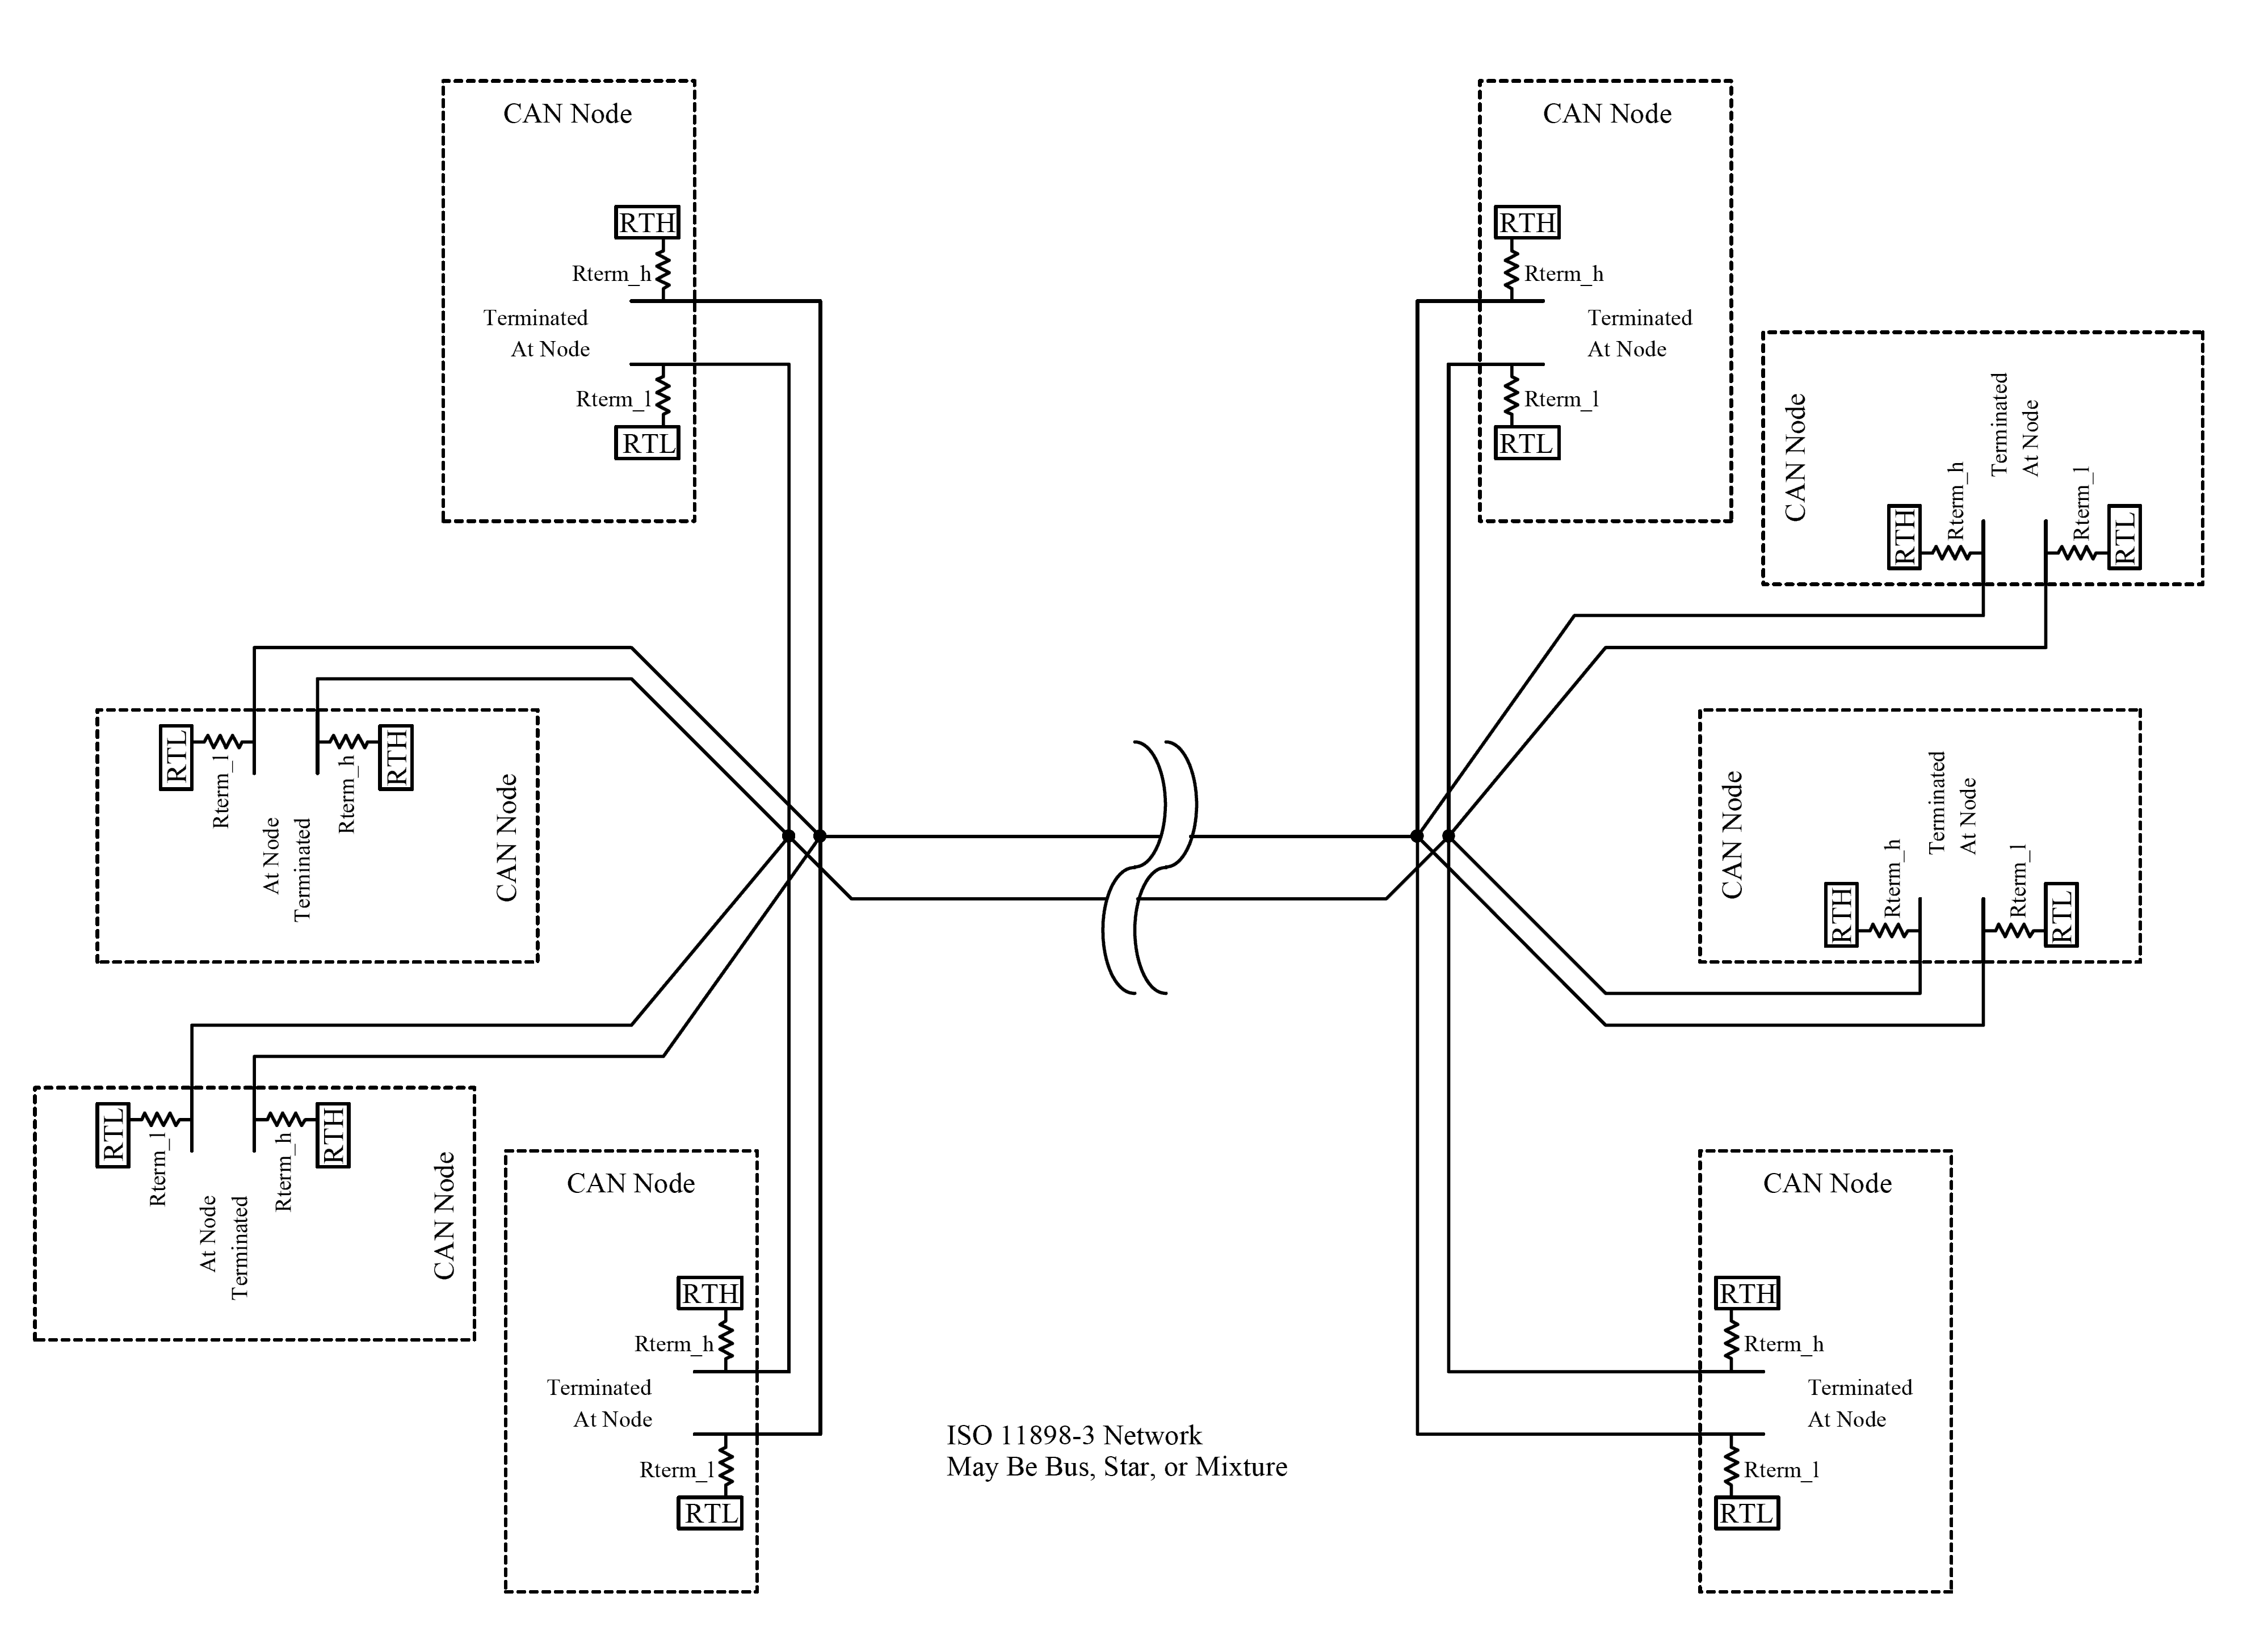
\includegraphics[width=.4\textwidth]{lowspeed.png}
% \caption{Low Speed CAN Network \cite{iso118983}}
% \end{figure}
% \end{frame}
%
% \subsection{Signalling}
% \begin{frame}
%   \frametitle{Bit Encoding}
%   \begin{itemize}
%     \item Level on bus can assume two complementary values:
%     \begin{itemize}
%       \item \textit{dominant}, usually corresponds to logical value 0
%       \item \textit{recessive}, usually corresponds to logical value 1
%     \end{itemize}
%     \item CAN relies on \emph{non-return to zero} (NRZ) bit encoding
%   \end{itemize}
%   \begin{figure}
%   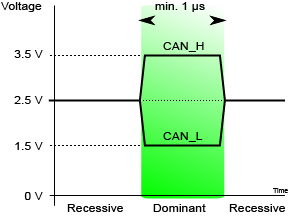
\includegraphics[width=.4\textwidth]{Canbus_levels.png}
% \caption{Levels on the CAN bus \cite{canlevels}}
% \end{figure}
% \end{frame}
%
% \begin{frame}
%   \frametitle{Synchronization}
%   \begin{itemize}
%     \item Timing information extracted from bit stream
%     \item Edges of the signal are used for synchronization
%     \item Bit stuffing to ensure sufficient number of edges
%   \end{itemize}
%     \begin{figure}
%   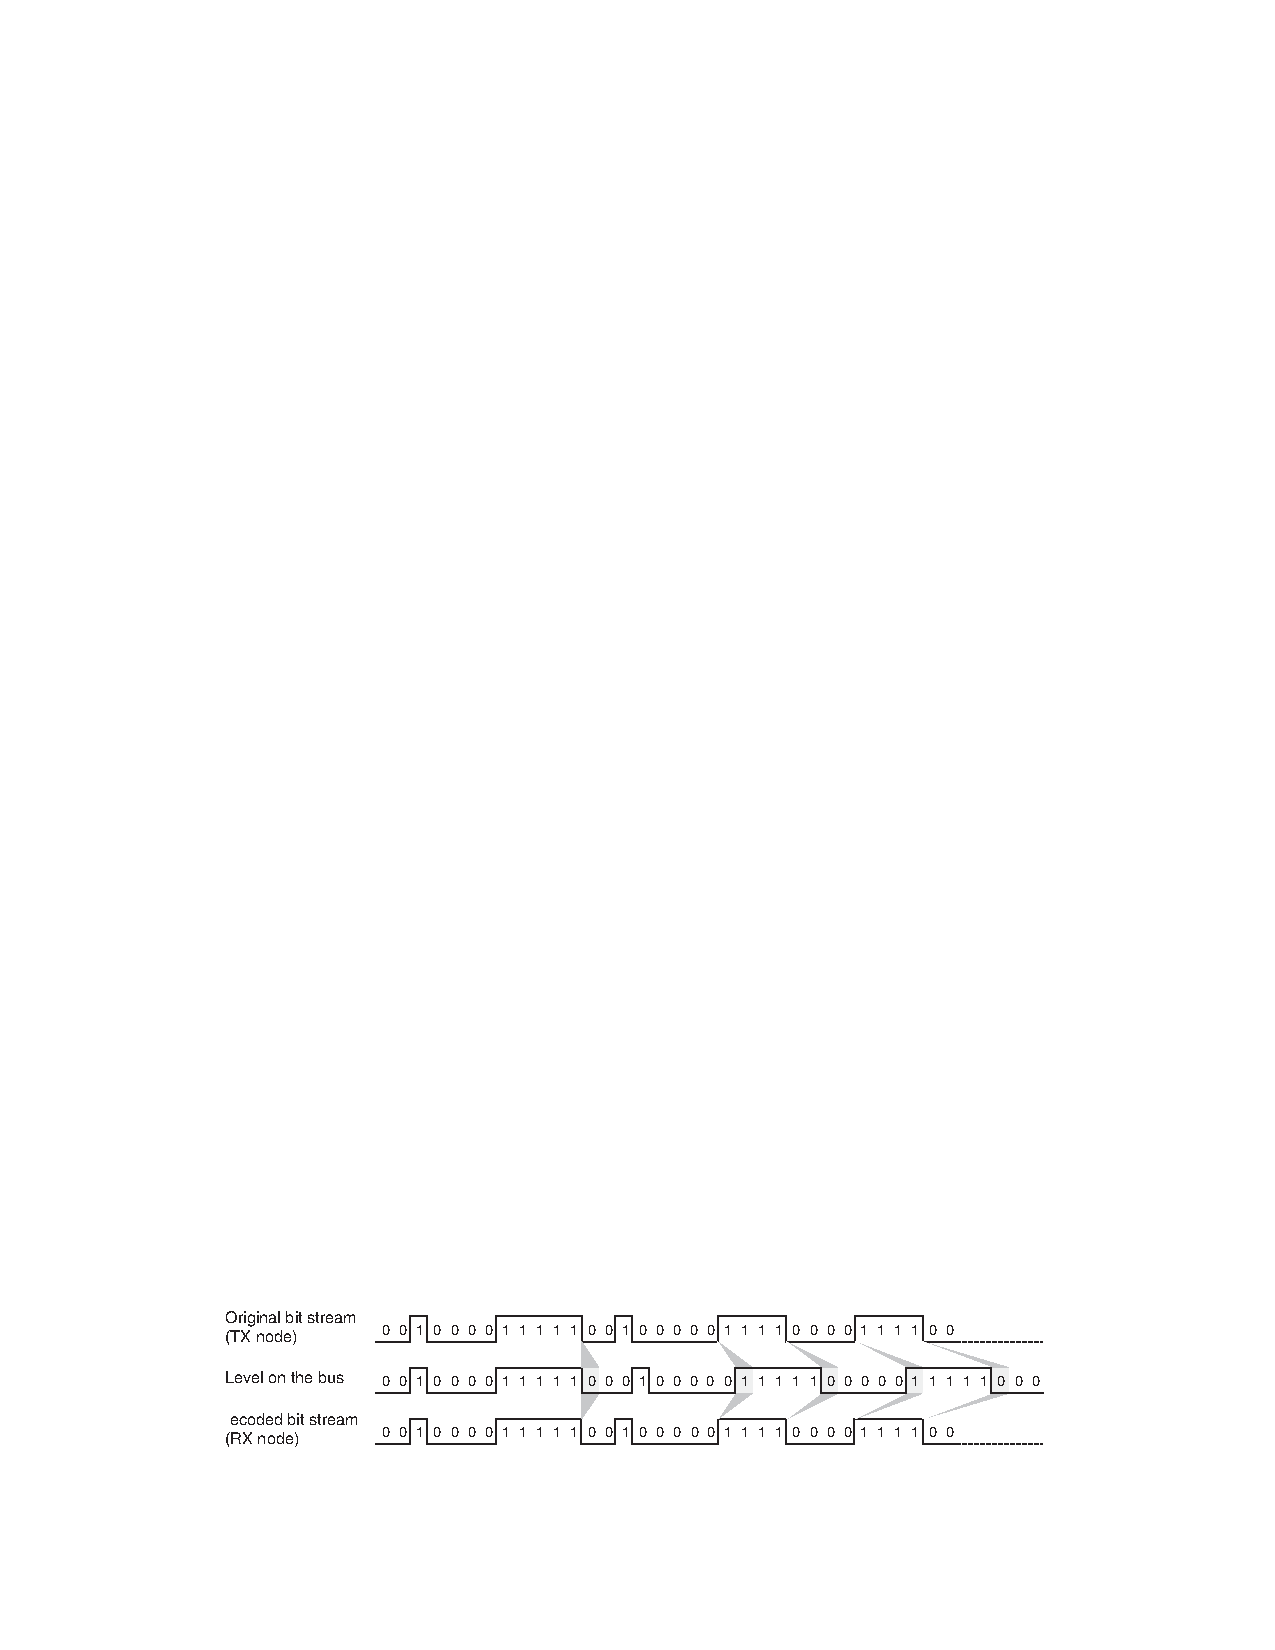
\includegraphics[width=.6\textwidth]{bitstuffing.pdf}
% \caption{Bit stuffing technique \cite{principles}}
% \end{figure}
% \end{frame}
%
% \section{Data Link Layer}
% \begin{frame}
%   \frametitle{Table of Contents}
%   \tableofcontents[currentsection]
% \end{frame}
% \subsection{Frame Format}
% \begin{frame}
%   \frametitle{Frame Format}
%   \begin{itemize}
%     \item Specifications define standard and extended frame format
%     \begin{itemize}
%       \item Standard: 11 bit identifier
%       \item Extended: 29 bit identifier
%     \end{itemize}
%     \item Standard frame format mostly used
%     \item Identifier describes meaning of message
%     \item Protocol foresees four kinds of frames: \emph{data, remote, error} and \emph{overload}
%   \end{itemize}
% \end{frame}
%
% \begin{frame}
%   \frametitle{Data Frames}
%   \begin{figure}
%     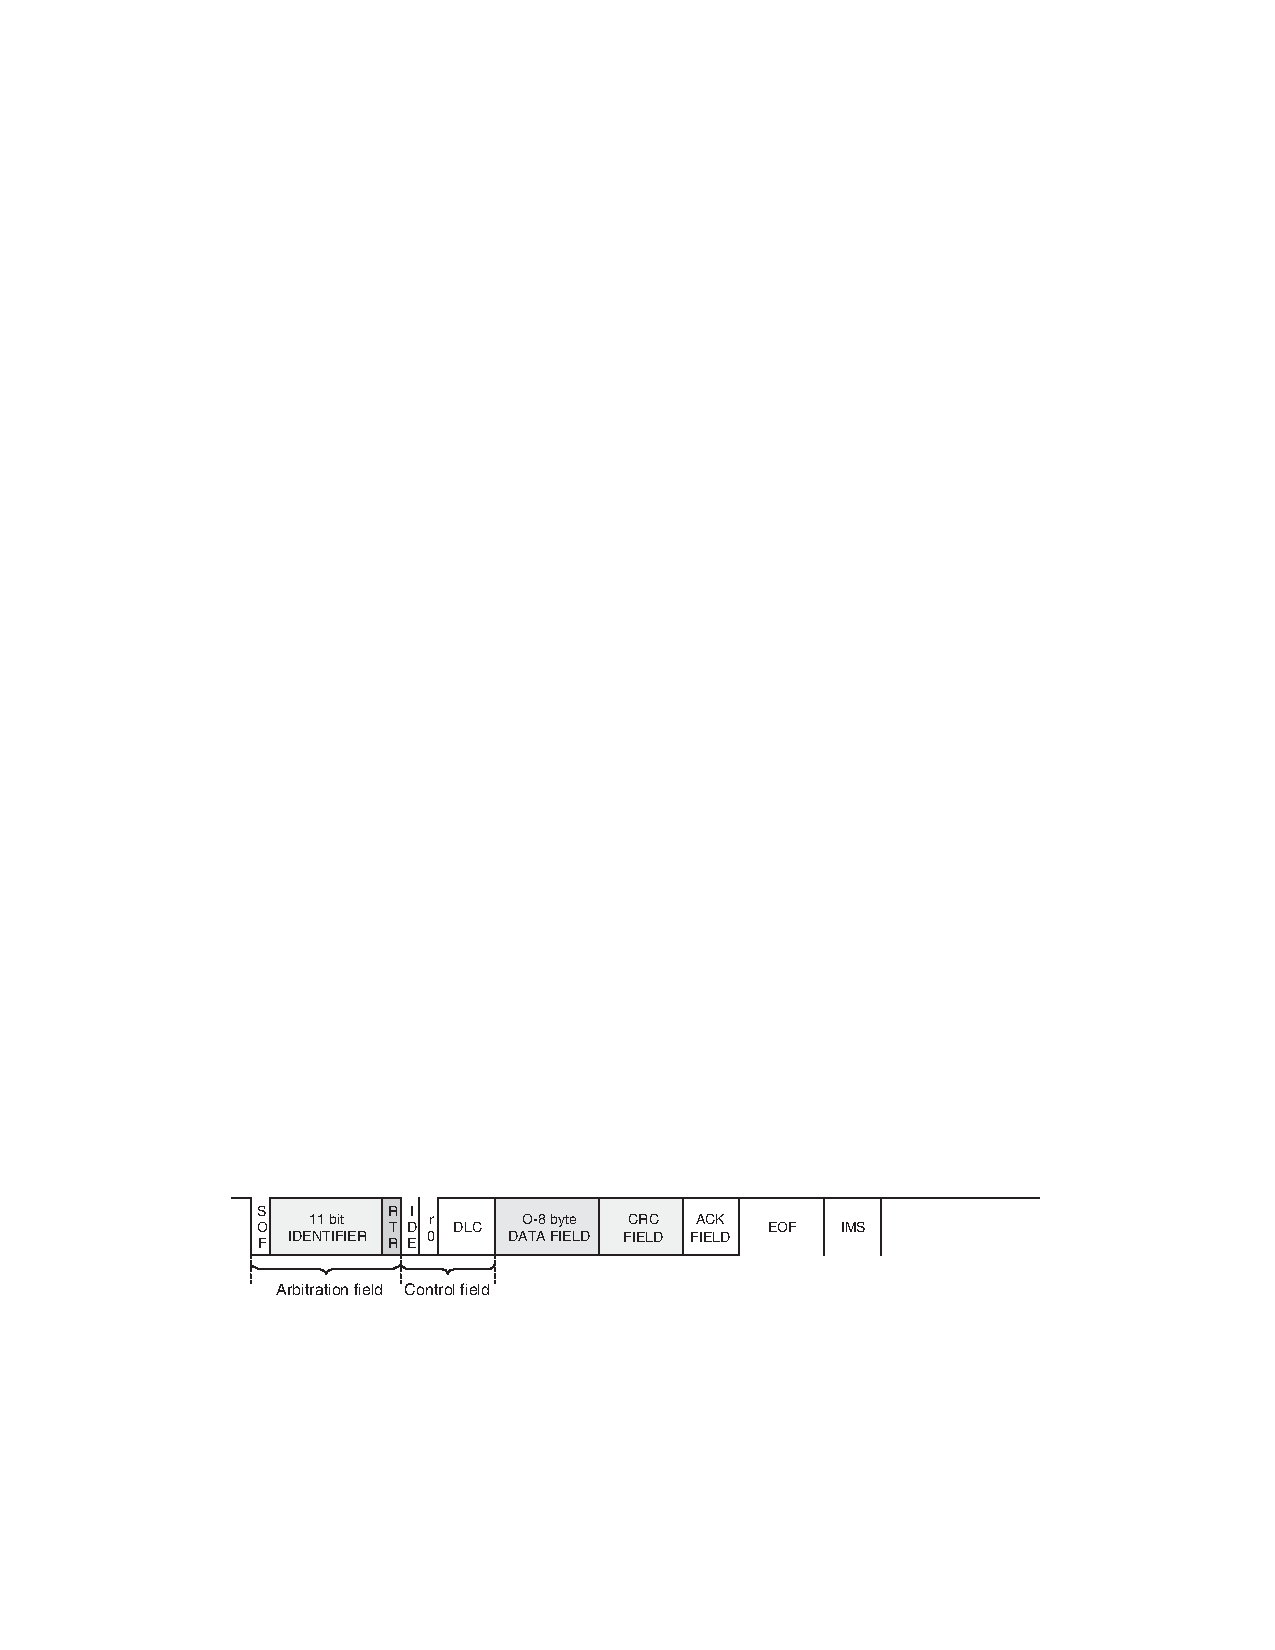
\includegraphics[width=.6\textwidth]{dataframe.pdf}
%     \caption{Format of standard data frames \cite{principles}}
%   \end{figure}
%   \begin{itemize}
%     \item Dominant \emph{start of frame} (SOF) bit
%     \item Arbitration field: identifier and \emph{remote transmission request} bit
%     \item \emph{Data length code} (DLC): Length of data field encoded in 4 bits
%     \item \emph{Cyclic redundancy check} (CRC) encoded in 15 bits
%     \item ACK slot: Recessive at transmitter, dominant at receiver
%     \item \emph{End of frame} (EOF) slot: Seven recessive bits
%   \end{itemize}
% \end{frame}
%
% \begin{frame}
%   \frametitle{Remote Frames}
%   \begin{itemize}
%     \item Generally, source sends out data autonomously
%     \item Protocol allows to poll for data
%     \item Remote format similar to data format
%     \item RTR field is recessive, data frames have higher priority
%     \item Remote frames carry no data
%   \end{itemize}
% \end{frame}
%
% \begin{frame}
%   \frametitle{Error Frames}
%   \begin{itemize}
%     \item Notify nodes that an error has occured
%     \item Consist of two fields:
%     \begin{itemize}
%       \item Error flag: Six dominant/recessive bits.\\
%         $\rightarrow$ Violates bit stuffing rules, error condition is detected
%       \item Error delimiter: 8 recessive bits.
%     \end{itemize}
%     \item Active flag: dominant, transmitted by node in state \emph{error active}
%     \item Passive flag: recessive, transmitted by node in state \emph{error passive}
%   \end{itemize}
% \end{frame}
%
% \begin{frame}
%   \frametitle{Fault Confinement}
%   \begin{itemize}
%     \item Supervises correct operation of MAC sublayer
%     \item Disconnect defective node from bus
%     \item Uses two counters: \emph{transmission} and \emph{receive error count}
%     \begin{itemize}
%       \item On error detect, counter is increased by a given amount
%       \item On success, counter is decreased by one
%       \item Increase amount of detecting node is higher than relying nodes
%     \end{itemize}
%     \item When counter exceeds 127, node switches from error active to error passive
%     \item When counter exceeds 255, node switches to bus off
%   \end{itemize}
% \end{frame}
%
% \begin{frame}
%   \frametitle{Overload Frames}
%   \begin{itemize}
%     \item Used to slow down operations on the bus by adding delays
%     \item Format similar to the error frames
%     \item Hardly ever used because today's CAN controllers are very fast
%   \end{itemize}
% \end{frame}
%
% \subsection{Access Technique}
% \begin{frame}
%   \frametitle{Access Technique}
%   \begin{itemize}
%     \item CAN relies on CSMA for access control:
%     \begin{itemize}
%       \item When no data is exchanged, level on the bus is recessive
%       \item Before transmission, nodes observe the state of the network
%       \item When network is idle, transmission starts immediately
%     \end{itemize}
%     \item Collisions are improbable but not impossible
%     \item CAN introduces collision resolution scheme: \textbf{Bus arbitration}
%   \end{itemize}
% \end{frame}
%
% \begin{frame}
%   \frametitle{CSMA/CR: Bus Arbitration}
%   Bus arbitration essentially identifies the most urgent frame.
%   \vfill
%   \begin{itemize}
%     \item Level on bus is dominant if one node is sending dominant bit
%     \item Nodes can reliably check level on bus
%     \item On transmission, each node compares level on bus against written value
%     \item If node transmits recessive bit but reads dominant, it backs off
%   \end{itemize}
% \end{frame}
%
% \begin{frame}
%   \frametitle{CSMA/CR: Bus Arbitration}
%   \begin{figure}
%     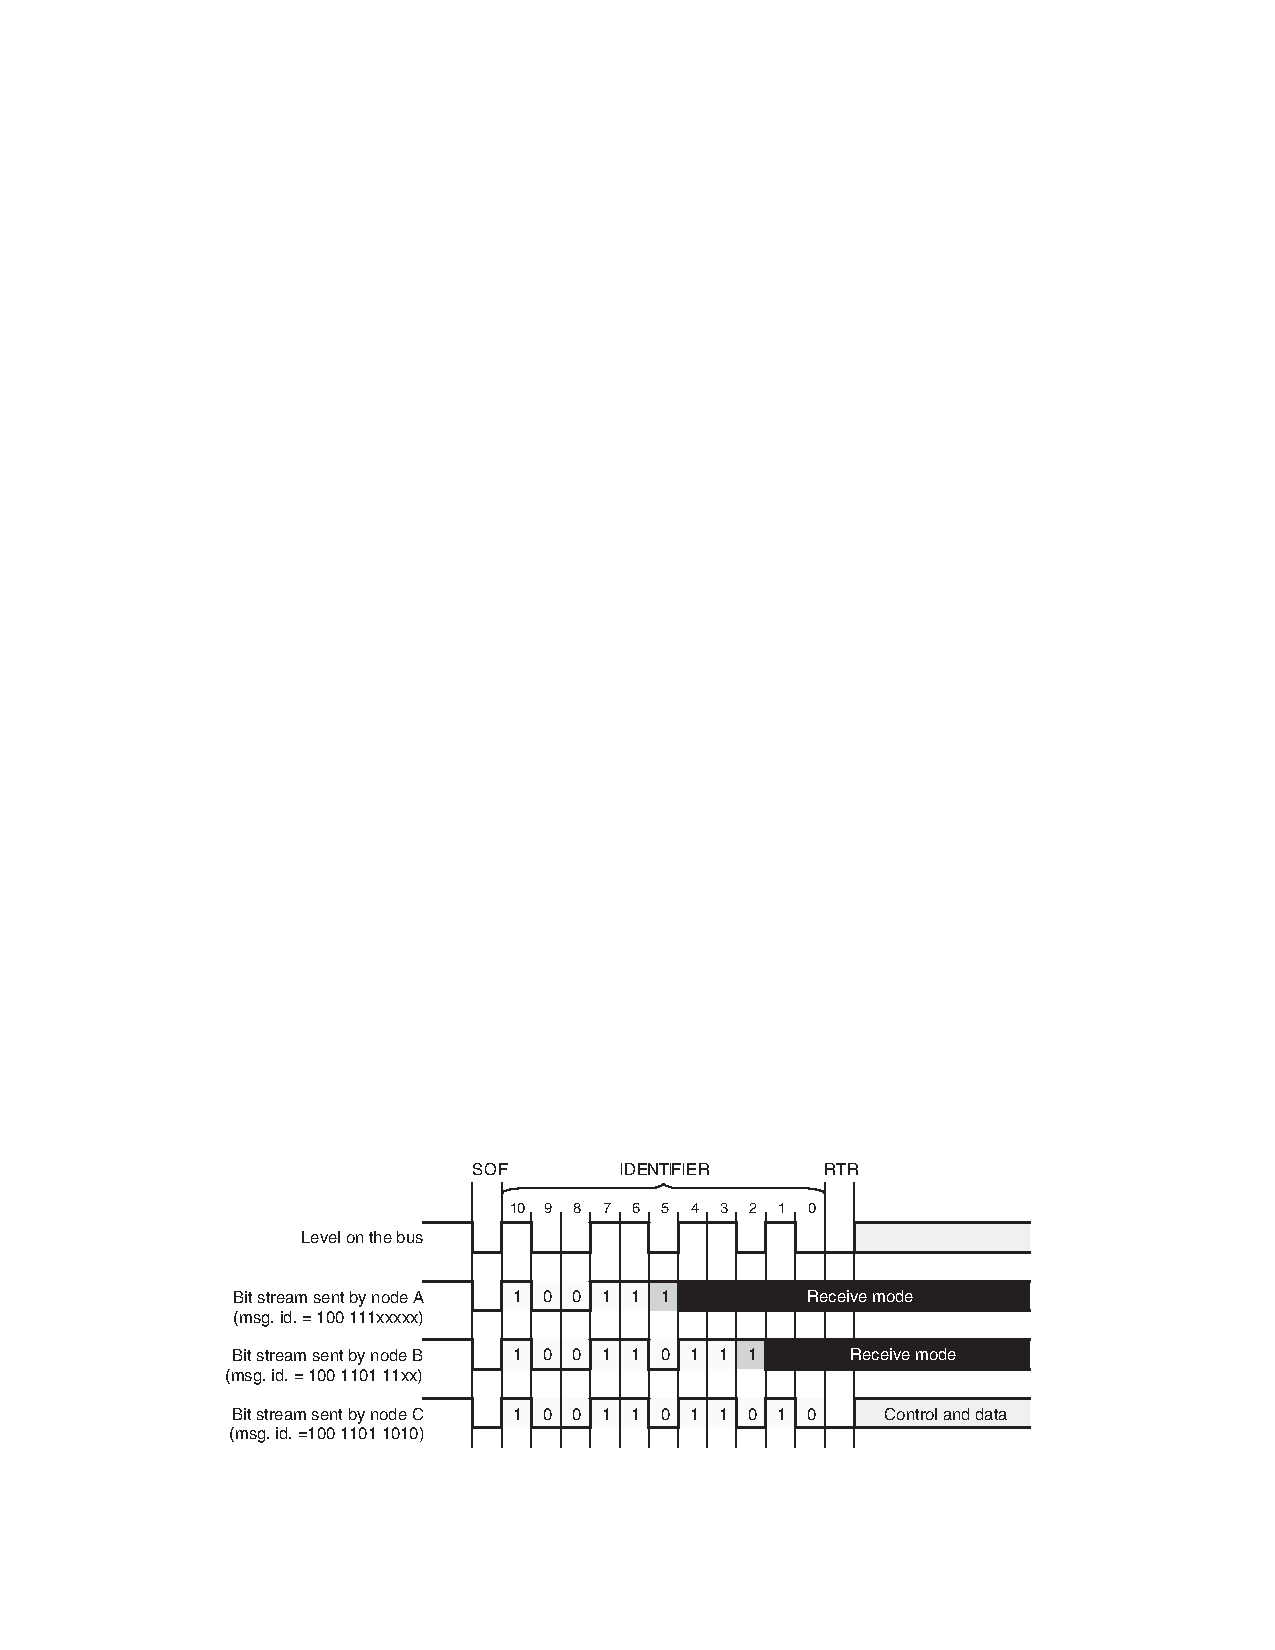
\includegraphics[width=.6\textwidth]{arbitration.pdf}
%     \caption{Arbitration phase in CAN}%Quelle
%   \end{figure}
%
%   \begin{itemize}
%     \item Nodes transmit message identifier starting with MSB
%     \item Lowest identifier corresponds to highest priority
%     \item Message with highest priority wins contention
%   \end{itemize}
% \end{frame}
%
% \subsection{Error Management}
% \begin{frame}
%   \frametitle{Error Management}
%   \begin{itemize}
%     \item Fundamental requirement for CAN is robustness
%     \item Specifications foresee five mechanisms for error detection:
%     \begin{itemize}
%       \item 15 bit wide CRC: Discover up to five erroneous bits
%       \item Frame check: CRC, ACK, EOF delimiters have to be recessive
%       \item Acknowledgement check: Transmitter checks for set ACK bit
%       \item Bit monitoring: Transmitter checks level on bus against written value
%       \item Bit stuffing: Each node verifies if bit stuffing rules have been violated
%     \end{itemize}
%     \item Residual probability for undetected corrupt message is $4.7 \cdot 10^{-11}$ times
%       the frame error rate or less
%   \end{itemize}
% \end{frame}
%
% \subsection{Communication Services}
% \begin{frame}
%   \frametitle{Logical Link Layer}
%   \begin{itemize}
%     \item Sublayer of Data Link Layer
%     \item Provides communication services to higher layers
%     \item Exports only two types of frames:
%     \begin{itemize}
%       \item \textbf{L\_DATA}: Broadcast value over the network
%       \item \textbf{L\_REMOTE}: Ask for value over the network
%     \end{itemize}
%     \item Error and overload frames invisible to higher layers
%     \item Provides \emph{frame acceptance filtering} function
%   \end{itemize}
% \end{frame}
%
% \begin{frame}
%   \frametitle{Frame Acceptance Filtering (FAF)}
%   \begin{itemize}
%     \item Producer transmits information on the bus
%     \item Frame is read by every node in a receive buffer
%     \item FAF determines if information is relevant to the node
%   \end{itemize}
%
%     \begin{figure}
%     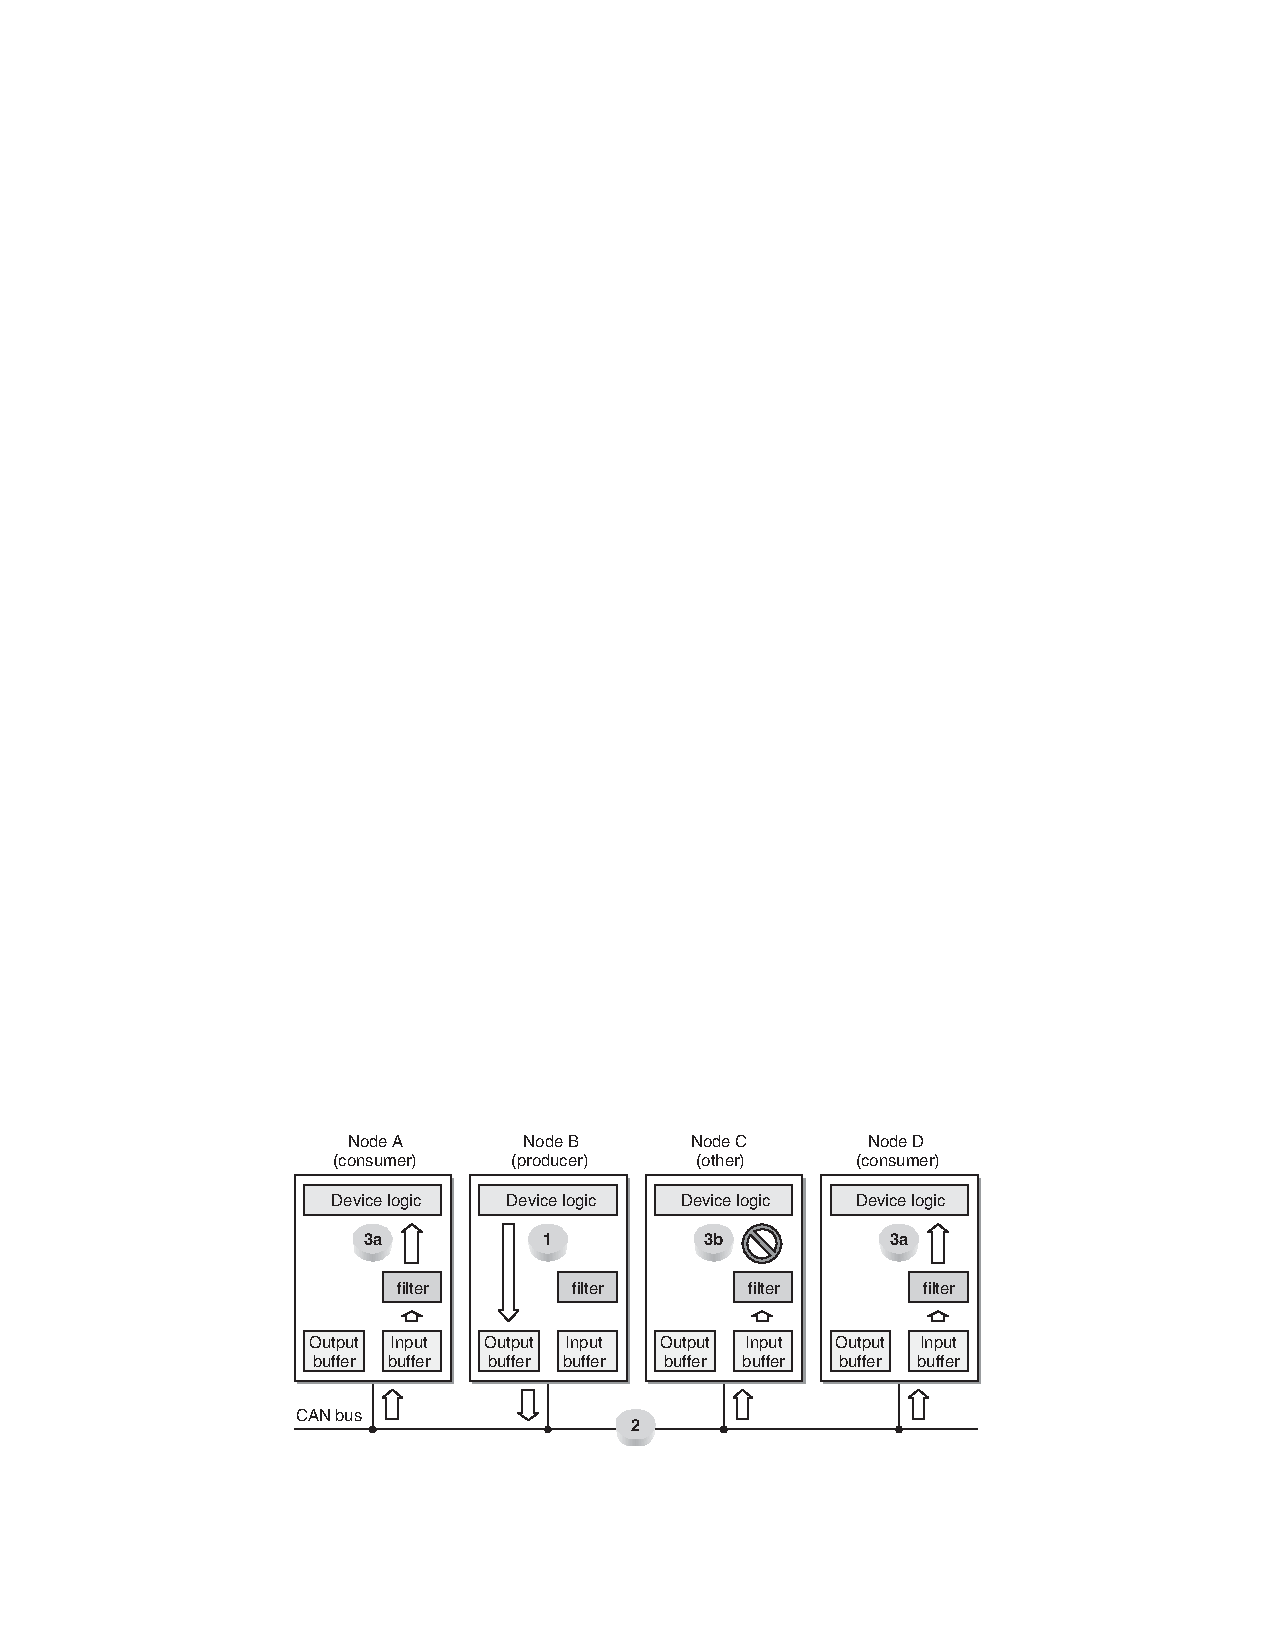
\includegraphics[width=.5\textwidth]{filtering.pdf}
%     \caption{Producer/consumer model}%Quelle
%   \end{figure}
% \end{frame}
%
%
% \section{Application Layer}
% \begin{frame}
%   \frametitle{Table of Contents}
%   \tableofcontents[currentsection]
% \end{frame}
% \subsection{CAN-based Application Protocols}
% \begin{frame}
%   \frametitle{Higher Layer Implementations}
%   \begin{itemize}
%     \item CAN specifications do not include application layer tasks
%     \begin{itemize}
%       \item Flow Control
%       \item Device Addressing
%       \item Fragmentation/Defragmentation
%     \end{itemize}
%     \item Several higher layer protocols rely on CAN
%     \item Industrial automation: CANopen, DeviceNet
%     \item Passenger cars: Each manufacturer has its own standard
%   \end{itemize}
% \end{frame}
%
% \section{Summary}
% \begin{frame}
%   \frametitle{Table of Contents}
%   \tableofcontents[currentsection]
% \end{frame}
% \subsection{Main Features of CAN}
% \begin{frame}
%   \frametitle{Advantages \& Disadvantages of CAN}
%   CAN implements a distributed priority-based multi-master communication system.
%   \vfill
%   \begin{itemize}
%     \item Advantages:
%     \begin{itemize}
%       \item Much more simple and robust than token based access schemes
%       \item More flexible than TDMA approaches
%       \item No message will be delayed by lower priority exchanges
%     \end{itemize}
%     \item Drawbacks:
%     \begin{itemize}
%       \item Relatively low maximum throughput
%       \item Bus length limited by bandwidth, arbitration, timing
%       \item Offers no security or authentication schemes
%     \end{itemize}
%   \end{itemize}
% \end{frame}
%
% \section*{Discussion}
% \begin{frame}
%   \frametitle{Thanks for your attention!}
%   \huge{Questions? Ideas? Suggestions?}
% \end{frame}
%
\section*{References}
\begin{frame}[allowframebreaks]
  \frametitle{References}
  \begin{thebibliography}{10}
  \beamertemplatebookbibitems
  \bibitem{profibusmanual}
    Max Felser
    \newblock Profibus Manual: A collection of information explaining PROFIBUS networks
    \newblock http://www.profibus.felser.ch
%   \bibitem{expanding}
%   Gabriel Leen, Donal Heffernan.
%   \newblock {\em Expanding Automotive Electronic Systems}
%   \beamertemplatearticlebibitems
%     \bibitem{iso118982}
%     EE JRW - Own work.
%     \newblock {\em CAN ISO11898-2 Network}.
%     \newblock Licensed under CC BY-SA 4.0 via Wikimedia Commons, 2015.
%     \newblock \url{http://commons.wikimedia.org/wiki/File:CAN_ISO11898-2_Network.png}
%     \bibitem{iso118983}
%     EE JRW - Own work.
%     \newblock {\em CAN ISO11898-3 Network}.
%     \newblock Licensed under CC BY-SA 4.0 via Wikimedia Commons, 2015.
%     \newblock \url{http://commons.wikimedia.org/wiki/File:CAN_ISO11898-3_Network.png}
%     \bibitem{canlevels}
%     Plupp - Own work.
%     \newblock {\em Canbus levels}.
%     \newblock Licensed under CC BY-SA 3.0 via Wikimedia Commons, 2015.
%     \newblock \url{http://commons.wikimedia.org/wiki/File:Canbus_levels.svg}
   \end{thebibliography}
 \end{frame}
\end{document}
